\chapter{Conclusão}
Nesse capítulo é apresentado como os testes foram organizados, as limitações do software, os resultados encontrados e futuras melhorias.

\section{Limitações}
Na criação do software os testes nos iniciais já possível identificar possíveis situações que o software não tem como dar uma resposta, ou seja, suas limitações.
Identificamos 3 possíveis limitações nos testes iniciais:  

\textbf{Não é possível entregar a tempo}: Levando em consideração o horário de saída e o horário limite para realizar todas as entregas, é possível que um percurso entre os endereços tem seu tempo de trajeto mais demorado que o tempo disponível para a realização de todas as entregas, com isso seria impossível entregar, mesmo com mais entregadores, com isso, o software não consegue definir uma rota por considerar a velocidade média das vias por onde ele passará.

\textbf{Limite de Entregadores:} Para pedir a definição de uma rota é preciso indicar quantos entregadores estão disponível para realizar as entregas, em algumas situações é possível que mesmo dividindo para todos os entregadores, mais entregadores seriam precisos para chegar a tempo em todos os endereços, com isso, o software não consegue definir uma rota.

\textbf{Tempo limite de entrega excedido:} Se a rota não tiver nenhum percurso muito demorado e também for possível determinar a divisão da rota principal entre o numero de entregadores, podemos encontrar outro problema, sempre que um entregador chega a um destino, é possível sofre atrasos na descarga, um maior tempo de espera ou até o transito piorando por causa de um acidente em uma via principal, por exemplo, isso muda o tempo dos próximos percursos, podendo elevar muito o tempo do trajeto.
É possível encontrar a situação que seria preciso mais entregadores para finalizar a entrega, que não é mais possível por que o entregador já está em transito, também pode encontrar um percurso completamente parado,  com isso, o software não consegue definir uma rota para finalizar as entregas.

\pagebreak
\section{Roteiros dos Testes}
Os roteiros foram escolhidos de forma arbitraria com endereços dentro ou próximos da cidade de São Paulo. As listas de endereços e as rotas encontrada podem ser vista a baixo:

O teste da tabela abaixo \ref{Roteiro1} começa o roteiro em Senac Nacões Unidas, endereço Av. Eng. Eusébio Stevaux, 823 - Santo Amaro, horário de saída 09:00, horário de volta 20:00, com 3 entregadores disponíveis e um tempo de espera médio em cada ponto 20 minutos.

\begin{table}[h]
	\centering
	\caption{Senac}
	\label{Roteiro1}
	\begin{tabular}{C{1cm}C{3cm}C{7cm}C{2cm}C{2cm}}
		\toprule
		\#&Nome&Endereço&Aber.&Fech.\\ \midrule
		1&Senac Largo Treze        & R. Dr. Antônio Bento, 393 - Santo Amaro                          & 09:00    & 12:00      \\
		2&Senac Taboão da Serra    & Rua Salvador Branco de Andrade, 182 - Jardim Sao Miguel          & 09:00    & 18:00      \\
		3&Senac Jabaquara          & Av. do Café, 298 - Jabaquara                                     & 09:00    & 11:00      \\
		4&Senac Osasco             & R. Dante Batiston, 248 - Centro                                  & 12:00    & 15:00      \\
		5&Senac Santana            & R. Voluntários da Pátria, 3167 - Santana                         & 10:00    & 19:00      \\
		6&Senac Tatuapé            & R. Cel. Luís Americano, 130 - Tatuapé                            & 15:00    & 19:00      \\
		7&Senac Vila Prudente      & Rua do Orfanato, 316 - Vila Prudente                             & 09:00    & 17:00      \\
		8&Senac - Campos do Jordão & Av. Frei Orestes Girardi, 3549 - Capivari, Campos do Jordão - SP & 09:00    & 17:00      \\ \bottomrule
	\end{tabular}
\end{table}

O calculo de rotas dividiu o roteiro para 2 entregadores, mesmo com varias tentativas para conseguir um melhor resultado, não foi possível encontrar uma rota para apenas um entregador, isso é pelo fato que, um dos endereço do roteiro fica em outra cidade, levando muito tempo para ir e voltar da entrega chegando no horário limite de volta para o deposito. Baixo um dos resultados encontrados para desse roteiro.

\begin{center}
	\makebox[\linewidth]{
		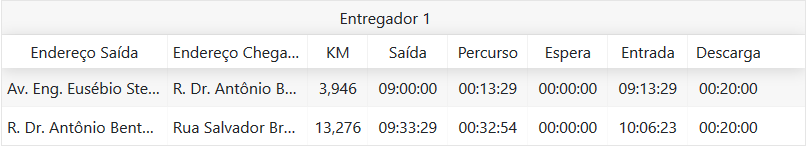
\includegraphics[keepaspectratio=true,scale=0.8]{ibagens/Senac-Entregador1.png}}
	\captionof{figure}{Resultado do Entregador 1}
	\label{fig:Senac-Entregador1}
\end{center}

\begin{center}
	\makebox[\linewidth]{
		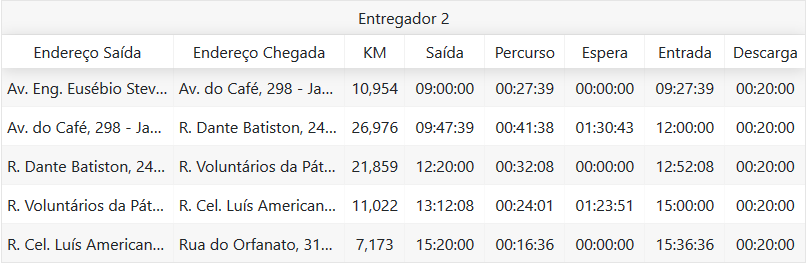
\includegraphics[keepaspectratio=true,scale=0.8]{ibagens/Senac-Entregador2.png}}
	\captionof{figure}{Resultado do Entregador 2}
	\label{fig:Senac-Entregador2}
\end{center}

\pagebreak
O teste da Tabela \ref{Roteiro2} começa o roteiro no Extra Morumbi, endereço Av. das Nações Unidas, 16741 - Santo Amaro, horário de saída 06:00, horário de volta 22:00:00, com 3 entregadores disponíveis e um tempo de espera médio em cada ponto 60 minutos.
\begin{table}[h]
	\centering
	\caption{Extra}
	\label{Roteiro2}
	\begin{tabular}{C{3cm}C{8cm}C{2cm}C{2cm}}
		\toprule
		Nome                     & Endereço                                                         & Aber. & Fech. \\ \midrule
		Extra Hipermercado       & R. João Batista de Oliveira, 47 - Centro, Taboão da Serra - SP     & 09:00    & 22:00      \\
		Extra João Dias          & Av. Guido Caloi, 25 - Jardim São Luís, São Paulo - SP              & 09:00    & 22:00      \\
		Extra Aeroporto          & Avenida Washignton Luís, 5859 - Jd. Aeroporto, São Paulo - SP      & 09:00    & 22:00      \\
		Extra - Itaim Bibi       & R. João Cachoeira, 899 - Itaim Bibi, São Paulo - SP                & 06:00    & 22:00      \\
		Extra - Ricardo Jafet    & Av. Dr. Ricardo Jafet, 1501 - Vila Mariana, São Paulo - SP         & 09:00    & 22:00      \\
		Extra                    & R. Nossa Sra. das Mercês, 29 - Vila das Merces, São Paulo - SP     & 09:00    & 22:00      \\
		Extra Hipermercado       & Av. Brigadeiro Luís Antônio, 2013 - Bela Vista, São Paulo - SP     & 09:00    & 22:00      \\
		Extra                    & Rua Três Rios, 282 - Bom Retiro, São Paulo - SP                    & 09:00    & 22:00      \\
		Extra Hiper Guarapiranga & Av. Guarapiranga, 752 - Socorro, São Paulo - SP                    & 09:00    & 22:00      \\
		Extra - Jardim Angela    & Estrada Velha do M'Boi Mirim, 4374 - Jardim Angela, São Paulo - SP & 09:00    & 22:00      \\
		Extra Hiper              & Av. Sen. Teotônio Vilela, 2926 - Jardim Iporanga, São Paulo - SP   & 09:00    & 22:00      \\ \bottomrule
	\end{tabular}
\end{table}

O calculo da rota encontrou um rota que pode ser feita por apenas um entregador, de forma que, não foi preciso utilizar todos os disponíveis. Os resultados completos estão nas tabelas abaixo.

\begin{center}
	\makebox[\linewidth]{
		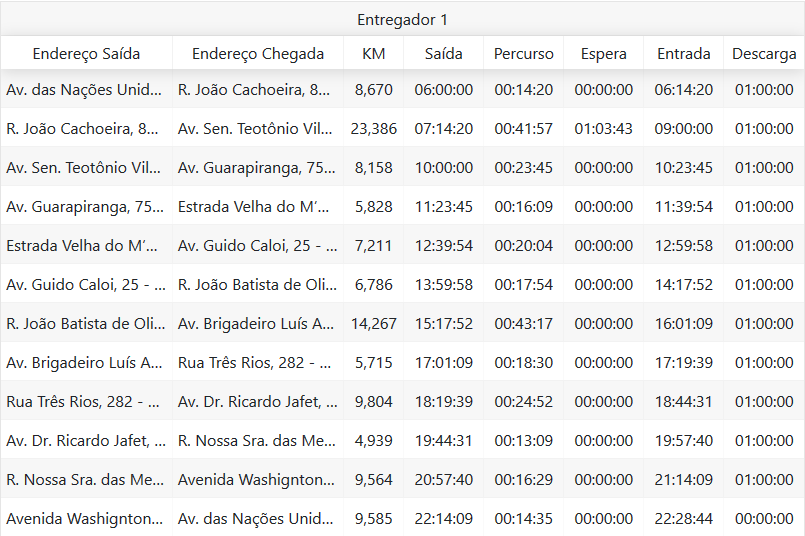
\includegraphics[keepaspectratio=true,scale=0.8]{ibagens/Extra-Entregador1.png}}
	\captionof{figure}{Resultado do Entregador 1}
	\label{fig:Extra-Entregador1}
\end{center}

\pagebreak
O teste da Tabela \ref{Roteiro3} começa o roteiro no McDonald's Jardim Paulista, endereço R. Pamplona, 734 - Jardim Paulista, São Paulo - SP, horário de saída 09:00, horário de volta 23:00, com 3 entregadores disponíveis e um tempo de espera médio em cada ponto 40 minutos.

\begin{table}[h]
	\centering
	\caption{MacDonald's}
	\label{Roteiro3}
	\begin{tabular}{C{3cm}C{8cm}C{2cm}C{2cm}}
		\toprule
		Nome                     & Endereço                                                         & Aber. & Fech. \\ \midrule
		McDonald's Augusta            & R. Augusta, 1856 - Cerqueira César, São Paulo - SP                                & 08:00    & 23:00      \\
		McDonald's Brigadeiro         & Av. Brigadeiro Luís Antônio, 3477/3481 - Jardim Paulista, São Paulo - SP          & 09:00    & 19:00      \\
		McDonald's José Maria         & Av. José Maria Whitaker, 81 - Jardim Paulista, São Paulo - SP                     & 09:00    & 21:00      \\
		McDonald's Nações Unidas      & Av. das Nações Unidas, 12555 - Pinheiros, São Paulo - SP                          & 06:00    & 21:00      \\
		McDonald's Eliseu de Almeida  & Av. Eliseu de Almeida, 2700 - Jardim Peri Peri, São Paulo - SP                    & 09:00    & 18:00      \\
		McDonald's Vital Brasil       & Av. Vital Brasil, 1256 - Butantã, São Paulo - SP                                  & 09:00    & 18:00      \\
		McDonald's Henrique Schaumann & Rua Henrique Schaumann, 80/124 - Cerqueira César, São Paulo - SP                  & 09:00    & 23:00      \\
		McDonald's Santo Antônio      & Av. Roque Petroni Júnior, 1089 - Chácara Santo Antônio (Zona Sul), São Paulo - SP & 09:00    & 23:00 \\ \bottomrule
	\end{tabular}
\end{table}
O calculo da rota dividiu o roteiro para apenas um entregador, de forma que, não foi preciso utilizar todos os 3 disponíveis. O resultado completo podem ser visto na tabela abaixo.

\begin{center}
	\makebox[\linewidth]{
		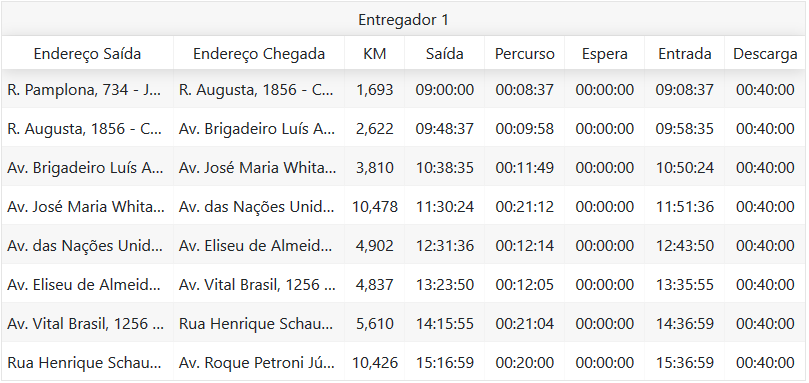
\includegraphics[keepaspectratio=true,scale=0.8]{ibagens/MacDonalts-Entregador1.png}}
	\captionof{figure}{Resultado do Entregador 1}
	\label{fig:MacDonalts-Entregador1}
\end{center}

\pagebreak
O teste da Tabela \ref{Roteiro4} começa o roteiro no Uninove Vergueiro, endereço Rua Vergueiro, 235/249 - Liberdade, São Paulo - SP, horário de saída 08:00, horário de volta 23:00:00, com 5 entregadores disponíveis e um tempo de espera médio em cada ponto 90 minutos.

\begin{table}[h]
	\centering
	\caption{Uninove}
	\label{Roteiro4}
	\begin{tabular}{C{3cm}C{8cm}C{2cm}C{2cm}}
		\toprule
		Nome                     & Endereço                                                         & Aber. & Fech. \\ \midrule
		Uninove Osasco                & R. Dante Batiston, 87 - Centro, Osasco - SP                                   & 08:00    & 23:00      \\
		Uninove Santo Amaro           & R. Amador Bueno - Santo Amaro, São Paulo - SP                                 & 08:00    & 23:00      \\
		Uninove São Bernardo do Campo & Av. Dom Jaime de Barros Câmara, 90 - Planalto, São Bernardo do Campo - SP     & 08:00    & 23:00      \\
		Uninove Vila Prudente         & Av. Professor Luiz Ignácio Anhaia Mello, 1363 - Vila Prudente, São Paulo - SP & 08:00    & 23:00      \\
		Uninove Vila Maria Baixa      & R. Itauna, 74 - Vila Maria Baixa, São Paulo - SP                              & 08:00    & 23:00      \\
		Uninove Barra Funda           & Av. Dr. Adolpho Pinto, 109 - Barra Funda, São Paulo - SP                      & 08:00    & 23:00      \\
		Uninove Mauá                  & R. Álvares Machado, 48 - Vila Bocaina, Mauá - SP                              & 08:00    & 23:00      \\
		Uninove Santo André           & R. Princesa Isabel - Vila Guiomar, Santo André - SP                           & 08:00    & 23:00 \\ \bottomrule
	\end{tabular}
\end{table}
O calculo da rota dividiu o roteiro para 2 dos 5 entregadores disponíveis. O resultado completo podem ser visto nas tabelas abaixo.

\begin{center}
	\makebox[\linewidth]{
		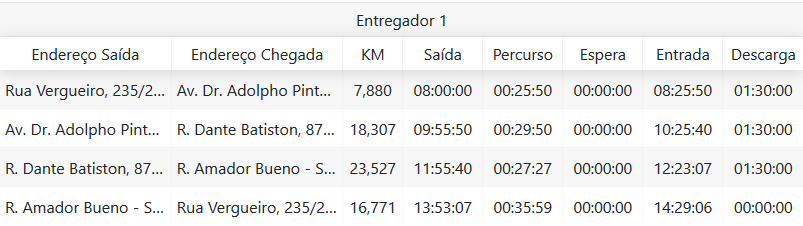
\includegraphics[keepaspectratio=true,scale=0.8]{ibagens/Uninove-Entregador1.png}}
	\captionof{figure}{Resultado do Entregador 1}
	\label{fig:Uninove-Entregador1}
\end{center}

\begin{center}
	\makebox[\linewidth]{
		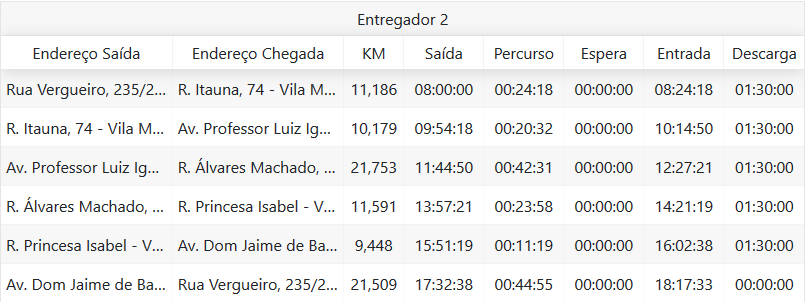
\includegraphics[keepaspectratio=true,scale=0.8]{ibagens/Uninove-Entregador2.png}}
	\captionof{figure}{Resultado do Entregador 2}
	\label{fig:Uninove-Entregador2}
\end{center}

\pagebreak
O teste da Tabela \ref{Roteiro5} simula a situação de 1 turista hospedado no Hotel Ibis São Paulo Paulista no endereço Av. Paulista, 2355 - Bela Vista, São Paulo - SP, em seu plano é conheço os endereços, permanecendo 30 minutos em cada, saindo do hotel 09:00 e voltando 23:00.

\begin{table}[h]
	\centering
	\caption{Pontos Turísticos de São Paulo}
	\label{Roteiro5}
	\begin{tabular}{C{3cm}C{8cm}C{2cm}C{2cm}}
		\toprule
		Nome                     & Endereço                                                         & Aber. & Fech. \\ \midrule
		Catedral Metropolitana de São Paulo & Praça da Sé - Sé, São Paulo - SP                                    & 00:00    & 23:59      \\
		Pte. Estaiada                       & Av. Jorn. Roberto Marinho, 85 - Cidade Monções, São Paulo - SP      & 00:00    & 23:59      \\
		Museu Catavento                     & Pq. Dom Pedro II - Av. Mercúrio, s/n - Brás, São Paulo - SP         & 09:00    & 16:00      \\
		Aquário de São Paulo                & R. Huet Bacelar, 407 - Ipiranga, São Paulo - SP                     & 09:00    & 17:00      \\
		Museu do Ipiranga                   & Parque da Independência - s/n - Ipiranga, São Paulo - SP            & 09:00    & 17:00      \\
		Parque Ibirapuera                   & Av. Pedro Álvares Cabral - Vila Mariana, São Paulo - SP             & 05:00    & 23:59      \\
		Zoológico De Sao Paulo              & Av. Miguel Estefno, 4241 - Vila Santo Estefano, São Paulo - SP      & 09:00    & 19:00      \\
		Jardim Botânico de São Paulo        & Av. Miguel Estefno, 3031 - Vila Água Funda, São Paulo - SP          & 09:00    & 17:00      \\
		Pateo do Collegio                   & Pç. Pateo do Collegio, 2 - Centro, São Paulo - SP                   & 09:00    & 16:30      \\
		Parque Estadual Alberto Löfgren     & R. do Horto, 931 - Horto Florestal, São Paulo - SP                  & 06:00    & 18:00      \\
		Parque Estadual do Jaraguá          & R. Antônio Cardoso Nogueira, 539 - Vila Chica Luisa, São Paulo - SP & 07:00    & 17:00      \\
		Autódromo de Interlagos             & Av. Sen. Teotônio Vilela, 261 - Interlagos, São Paulo - SP          & 07:00    & 17:00      \\
		Anhembi Sambadrome                  & Av. Olavo Fontoura, 1209 - Santana, São Paulo - SP                  & 07:00    & 17:00 \\ \bottomrule
	\end{tabular}
\end{table}

Mesmo com varias tentativas, o calculador de rotas não encontrou um rota onde seria possível com apenas uma pessoa em um dia, visitar todos os endereços do roteiro. Alterando para um tempo de permanência menor de 30 minutos, depois de varias tentaria, foi possível obter um resultado que pode ser visto a baixo.

\begin{center}
	\makebox[\linewidth]{
		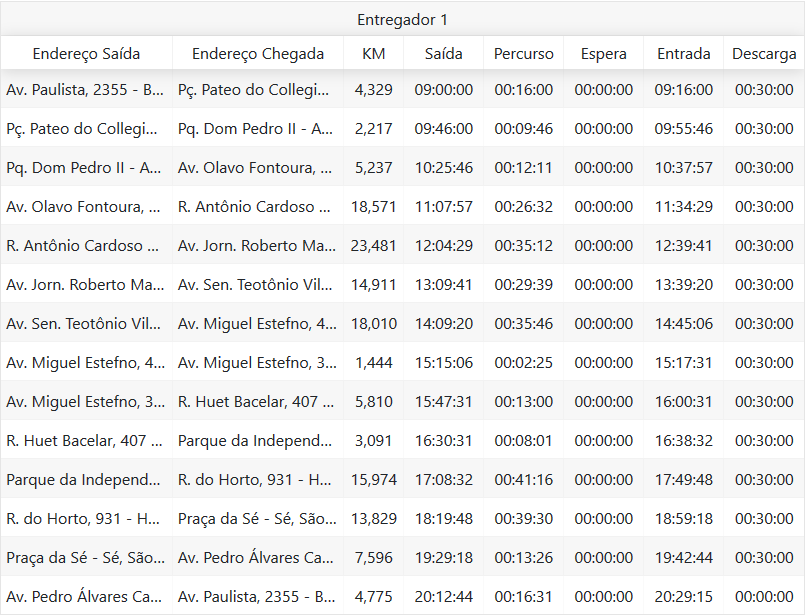
\includegraphics[keepaspectratio=true,scale=0.8]{ibagens/Turista.png}}
	\captionof{figure}{Resultado do Turista}
	\label{fig:Turista}
\end{center}

Mesmo com o foco em entregas, o software poderia ser utilizado para outras funções, mesmo parecendo simples encontrar um roteiro que de para ver todos os pontos de interesse, se torna um trabalho complicado com você tem horários e tempo de percurso. O software por utilizar GA para encontrar a rota, teve dificuldade para encontrar uma rota que seria possível para apenas uma pessoa passar por todos esses lugares.

\pagebreak
\section{Comparativo}
O software se mostrou eficiente para entrar uma rota que minimiza o numero de entregadores e respeitando os horários de cada endereço. Roteiros que, a primeira vista, parecem impossíveis de ser entregue, rotas foram encontradas e organizadas.
O Google Maps ajuda na definição da rota por entregar o transito médio da rota fazendo com que o caminho escolhido pelo software fique mais próximo de uma situação real. 

O GA ajuda na escolhas das rotas por exemplo tentar minimizar o tempo, a distância e o numero de entregadores, encontrando padrões difíceis de ser vistos, porém, para encontrar uma solução próxima do ótimo é preciso perder performance para calcular a resposta, aumentando o numero de gerações e população para encontrar a rota.

Utilizando um numero baixo de destinos o processo de recalculo de rotas para cada vez que chegar em um  destino, se mostra útil para identificar mudanças no transito e ainda chegar no horário proposto. Em casos que é preciso calcular para muitos destinos,é mais recomendado somente utilizar para uma divisão de tarefas ou pré-analise do roteiro, por tornar a analise muito demora, o tamanho da população e numero de gerações precisa ser mais altos para melhor precisão dos resultados.

Para comparativo foi utilizado os diferentes tipos de mutação e cruzamentos, de forma, a identificar uma melhor combinação para ser utilizada no software, 10 vezes para cada combinação utilizando a média do valor do valor de aptidão. A tabela abaixo estão os resultados encontrados:

\pagebreak
\begin{table}[h]
	\centering
	\caption{Comparação dos Cruzamentos e Mutações}
	\label{Comparacao}
	\begin{tabular}{C{2.5cm}C{1.5cm}C{1.5cm}C{1.5cm}C{1.5cm}C{1.5cm}C{1.5cm}}
		\hline
		\textbf{Extras.txt}               & \textbf{EM} & \textbf{DIVM} & \textbf{DM} & \textbf{IM} & \textbf{IVM} & \multicolumn{1}{l|}{\textbf{SM}} \\ \hline
		\multicolumn{1}{l|}{\textbf{OBX}} & 109560      & 109560        & 109560      & 109560      & 109560       & 109560                           \\
		\multicolumn{1}{l|}{\textbf{PBX}} & 109560      & 109560        & 109560      & 109560      & 109560       & 109560                           \\
		&             &               &             &             &              &                                  \\ \hline
		\textbf{MacDonalts.txt}           & \textbf{EM} & \textbf{DIVM} & \textbf{DM} & \textbf{IM} & \textbf{IVM} & \textbf{SM}                      \\ \hline
		\multicolumn{1}{l|}{\textbf{OBX}} & 43320       & 43320         & 43320       & 43320       & 43320        & 43320                            \\
		\multicolumn{1}{l|}{\textbf{PBX}} & 43320       & 43320         & 43320       & 43320       & 43320        & 43320                            \\
		&             &               &             &             &              &                                  \\ \hline
		\textbf{Senacs.txt}               & \textbf{EM} & \textbf{DIVM} & \textbf{DM} & \textbf{IM} & \textbf{IVM} & \textbf{SM}                      \\ \hline
		\multicolumn{1}{l|}{\textbf{OBX}} & 311876      & 311876        & 311876      & 311876      & 311876       & 311876                           \\
		\multicolumn{1}{l|}{\textbf{PBX}} & 311876      & 311876        & 311876      & 311876      & 311876       & 311876                           \\
		\textbf{}                         &             &               &             &             &              &                                  \\ \hline
		\textbf{Uninoves.txt}             & \textbf{EM} & \textbf{DIVM} & \textbf{DM} & \textbf{IM} & \textbf{IVM} & \textbf{SM}                      \\ \hline
		\multicolumn{1}{l|}{\textbf{OBX}} & 190656      & 190656        & 190656      & 190656      & 190656       & 190656                           \\
		\multicolumn{1}{l|}{\textbf{PBX}} & 190656      & 190656        & 190656      & 190656      & 190656       & 190656                           \\
		\textbf{}                         &             &               &             &             &              &                                  \\ \hline
		\textbf{Turisticos.txt}           & \textbf{EM} & \textbf{DIVM} & \textbf{DM} & \textbf{IM} & \textbf{IVM} & \textbf{SM}                      \\ \hline
		\multicolumn{1}{l|}{\textbf{OBX}} & 84573       & 84573         & 84573       & 84573       & 84573        & 84573                            \\
		\multicolumn{1}{l|}{\textbf{PBX}} & 84573       & 84573         & 84573       & 84573       & 84573        & 84573                           
	\end{tabular}
\end{table}

Como mostrado na tabela \ref{Comparacao}, a mutação ou cruzamento escolhida não influencia no resultado, apresentando o mesmo valor de aptidão para todas as combinações em nos diferentes roteiros.


\section{Trabalhos futuros}

Devido a média de tempo para se encontrar as rotas, avaliar a possível paralelização da rotina de algoritmos genéticos para tornar o projeto viável para uso em uma aplicação web.
Avaliar a aplicação de heurísticas  \(\lambda-interchange\), \textit{k-node}, \textit{Or-opt} no calculo do \textit{Fitness}.
Utilizar uma base de dados maior para os testes, baseada em casos reais de logística.
Criar uma aplicação web para utilização em um caso real de entregas.




